\documentclass[justified,notitlepage]{tufte-book}   	
% use "amsart" instead of "article" for AMSLaTeX format
%\usepackage{geometry}                		% See geometry.pdf to learn the layout options. There are lots.
%\geometry{letterpaper}                   		% ... or a4paper or a5paper or ... 
%\geometry{landscape}                		% Activate for for rotated page geometry
%\usepackage[parfill]{parskip}    		% Activate to begin paragraphs with an empty line rather than an indent
\usepackage{appendix}
\usepackage{graphicx}				% Use pdf, png, jpg, or eps with pdflatex; use eps in DVI mode
\usepackage[plain]{fancyref}								% TeX will automatically convert eps --> pdf in pdflate
\usepackage{amsmath}
\usepackage{mathtools}	
\usepackage{amssymb}
\usepackage{amsthm}

%\newcommand*{\fancyrefthmlabelprefix}{eq}
\newcommand*{\fancyrefthmlabelprefix}{thm}
\frefformat{plain}{\fancyrefthmlabelprefix}{theorem~#1}
\Frefformat{plain}{\fancyrefthmlabelprefix}{Theorem~#1}
\newcommand*{\fancyrefapplabelprefix}{app}
\frefformat{plain}{\fancyrefapplabelprefix}{appendix~#1}
\Frefformat{plain}{\fancyrefapplabelprefix}{Appendix~#1}
\title{Optimal Population Coding of Dynamic Stimuli}
\author{Alex Kunze Susemihl}
%\date{}							% Activate to display a given date or no date

\begin{document}
\maketitle
\setcounter{secnumdepth}{1}
\tableofcontents
\chapter{Introduction}

\newthought{Neuroscience as a whole} is concerned with the function of the nervous system. More precisely, it asks a very simple question: {\em What is the brain 
doing?}\footnote{ Or alternatively: {\em What is the nervous system doing?}} The simplicity with which humans and animals perform in their environment makes it 
almost unnatural to ask how their brains enable these behaviors. It is often hard to explain to laymen the complexity involved in preparing even the simplest actions, 
such as saccades or walking, such is the ease with which these are normally performed. Although one can not realistically expect to answer that question in any 
general fashion, I will try to touch upon a number of points which shed light on some aspects of the nervous system and provide us with a {\em guiding principle} to 
understand what the brain is doing, why and possibly how.\par

Neuroscience was born as a branch of biology, and although it is now often thought of as  an interdisciplinary science in itself, its objects of study are still to the 
largest extent biological systems. Theodosius Dobzhansky published an influential essay in 1973, entitled {\em Nothing in biology makes sense except in the light of 
evolution},\cite{Dobzhansky1973} which defends exactly that point. Though it has been reviewed and revisited constantly since its proposal, the theory of evolution 
through natural selection remains the central pillar of biological sciences. As such, neuroscience must also view its objects of study through the lenses of evolution. 
More specifically, we can then ask ourselves {\em What evolutionary advantage would this brain bring to an individual?} instead of {\em Why is the brain this way?} 
That being said,  there are caveats in the case of neuroscience. For one, the brain is capable of plasticity and adaptation unthinkable for other organs, and so we can 
not expect to understand the functionality of the brain in the same way in which the shape of bird beaks can be understood as a function of their preferred fruits and 
seeds. Furthermore, the brain controls all of the motor and perceptual apparatus, having a multitude of uses and purposes, unlike simpler organs.\par

One particular aspect of the brain which has received increasing attention recently is its ability to deal with uncertainty. In a very fruitful line of research, a number 
of experiments have demonstrated that humans and animals integrate uncertain information in a near-optimal way. The so-called {\em Bayesian Brain},\cite{Knill2004} 
would explicitly represent the distribution over world states and perform inference in a manner consistent with Bayesian inference, obtaining optimal integration of 
sensory cues from different modalities, for example. It is still a matter of debate how these Bayesian computations would be implemented in the brain. One possibility 
is that the activity of neurons is sampling from a representation of the distribution of world states,\cite{Berkes2011} which is frequently called the {\em sampling 
hypothesis}. Another is that the activity of the neurons itself represents the likelihood over world states,\cite{Ma2006} and the population as a whole codes for the 
distribution, hence the term {\em population coding}.\par

\subsection*{Structure}

\newthought{The main goal of this thesis} is to develop a conceptual framework for studying optimal population coding in a dynamic framework. Furthermore, I will
establish a link between optimal dynamic encoders and the efficient coding hypothesis, first proposed by Horace Barlow.\cite{Barlow1961} I believe that the 
inclusion of time into the coding framework raises a number of questions, which have not been addressed in the scientific literature properly. In the remainder of this 
chapter, I will discuss the efficient coding hypothesis and its more recent developments, and I will touch upon its relationship to Shannon's information theory.\cite{Shannon1948} I will finish by discussing the issue of dynamic population coding, highlighting the issues which I believe are of importance in considering the 
temporal aspect of coding. I will make the case for a study of optimal filtering of partially observed stimuli as a model of stimulus inference based on spike trains. 
Following, in \fref{chap:filtering}  I will introduce the general theory of filtering of stochastic stimuli. After that, in \fref{chap:MSE} I will discuss results regarding the 
Mean-Squared-Error (MSE) of optimal filters of point process data, presenting a number of new analytical results. In \fref{chap:control}, I will generalize the filtering 
framework to control problems, showing results for optimal control theory of point process-observed processes. In \fref{chap:optimal} I will then provide the connection 
to neuroscience, by considering the optimal encoding strategy for a population of neurons coding for a stochastic stimulus. I will then finalize by discussing the impact 
of the work presented and suggesting future research directions.\par

\subsection*{Contribution}

\newthought{The main contribution of this thesis} is in providing a conceptual toolbox to study optimal coding problems in a dynamic environment. I propose that the 
study of the average performance of an optimal Bayesian filter reconstructing the relevant stimulus provides a good measure of the quality of a dynamic code. Using 
this framework, I derive analytical results for the fast population code for dense populations of Gaussian neurons proposed by Quentin Huys.\cite{Huys2007} These are 
to my best knowledge the first results of this kind obtained for temporal coding of dynamic stimuli.\par

The results presented in this thesis have been published and presented throughout the duration of my doctoral studies. The findings in \fref{chap:MSE} were first
published at the \emph{Neural Information Processing Systems} conference, where it was presented as a poster in addition to the publication in the conference 
proceedings \citep{Susemihl2011a}. These results were then further developed and put in the greater context of computational neuroscience and published in a special
edition of the \emph{Journal of Statistical Mechanics: Theory and Experiment} title \emph{Statistical Physics and Neuroscience}, focusing on the challenges 
neuroscience presented to statistical physics \citep{Susemihl2012a}. The results presented \fref{chap:control} have been submitted to the \emph{NIPS} conference
proceedings as well, and are currently under review.\par

Parallelly to the topics presented here I have also contributed to other ongoing research projects during my doctoral studies. In a research project headed by 
fellow doctoral student Chris H\"ausler and myself, we have proposed a novel way of training temporal Boltzmann machines, which improves their performance as
generative models of temporal data greatly. This was presented in a workshop on Deep Learning at the \emph{NIPS} conference as well \citep{hausler2012b}. This was
then used as a model for temporal sparsity in visual cortex and results on sequences of natural images were published in the journal \emph{Brain Research} in a
special issue on neural coding \citep{Hausler2013a}. The advantages of the training procedure for generative models of temporal data as well as for forecasting were
further extended on and submitted for publication in the journal \emph{Neurocomputing} \citep{Hausler2013b}.\par

In addition to these projects, I have also worked on the publication of a manuscript originating from my Masters thesis, which was since published in the journal 
\emph{Physica A}. There we investigated the effect of different learning strategies on the emergence of moral opinions in a model of social learning  
\citep{Vicente2014}.

\section{Efficient Coding Hypothesis}

\newthought{In information theory, the information} associated with a random event is defined as the logarithm of its inverse probability. We can further define the 
entropy of a distribution 
over a set of events as the average information conveyed by these events. So if we have a random variable $X$ taking values $x \in \mathcal{A}_X$ and a probability 
distribution $P_X : \mathcal{A}_X \to [0,1]$, we will have\footnote{Abusing the notation to allow for $0\log(0) = 0$.}
$$
H(X)= \sum_x P_X(x) \log\left(\frac{1}{P_X(x)}\right) = - \sum_x P_X(x) \log\left({P_X(x)}\right).
$$
The entropy measures how much information is gained from a random observation of $X$ on average, and is usually thought of as a measure of the uncertainty or 
disorder in the distribution $P_X$. Its unit is usually defined as the {\em bit} when the logarithm is taken in base 2, contracted from \emph{binary digit}. So, a distribution where 
we have $P_X(x^*) = 1$ for some $x^*$ and $P_X(x) = 0$ for all other $x\neq x^*$ would have an entropy of $0$, since our measurement gives us an average 
information of $0$. The outcome $x^*$ is completely non-informative, and all other outcomes, while infinitely informative have a zero probability of happening.\par
It can also easily be seen that in the absence of other constraints, if the set of outcomes $\mathcal{A}_X$ is finite, the entropy is maximized by the uniform 
distribution over outcomes $x$, which would give us the maximal average information per observation of the variable $X$.\footnote{We provide a short demonstration in 
\fref{app:entropy}} In information theory, the entropy provides the number of bits it takes, on average, to specify an outcome of the random variable $X$.\par
We can now define the conditional entropy of two random variables $X$ and $Y$ as
$$
H(Y|X) = \sum_x P_X(x) \sum_y P_Y(y|x) \log\left(\frac{1}{P_Y(y|x)}\right),
$$
i.e. the conditional entropy is the average entropy of $Y$ given $X$, averaged over $X$. This gives us the remaining uncertainty in $Y$ after $X$ has been observed averaged over all outcomes of $X$, or alternatively, the number of bits required to code for an outcome of $Y$ given an outcome of $X$, on average. Let us also define the mutual information between $Y$ and $X$ as
$$
I(X;Y) = H(Y) - H(Y|X) = H(X) - H(X|Y) = I(Y;X).
$$
In line with our interpretation of the conditional entropy, this would give us the average reduction of uncertainty in $Y$ given the observation of $X$ or vice-versa. Note that, if we fix the distribution of $X$ (or $Y$), the mutual information is always maximized if the conditional entropy $H(X|Y)$ (or $H(Y|X)$, respectively) is minimized. It is easy to see that if $P_X(x|y)$ ($P_Y(y|x)$) is given by a one-to-one mapping between $X$ and $Y$, the conditional entropy is zero, as no uncertainty is left in $X$ after the observation of $Y$ (no uncertainty in $Y$ is left after the observation of $X$).\par
Shannon regarded a noisy communication channel as a set of two random variables, one representing the codeword to be transmitted ($X$) and another representing the message received ($Y$). The noise in the channel would then be given by the conditional distribution of received messages given the transmitted codewords ($P_Y(y|x)$). The capacity of this channel is then given by
$$
C = \max_{P_X} I(X;Y).
$$
This is the maximum amount of information we can transmit through a noisy channel given by the distribution $P_Y(Y|X)$.
The rate of a given code is given by the number of bits needed to represent $X$ divided by the number of bits needed to represent $Y$, so if to send a one-bit message $x$ we must transmit a three-bit codeword $y$, our code would have a rate of $1/3$.
The noisy-channel coding theorem\cite{mackay2003information} then states
\newtheorem{noisychannel}{Theorem}
\begin{noisychannel}
\label{thm:noisychannel}
For every discrete memoryless channel with capacity $C$, for any $\epsilon>0$, any rate $R<C$, and for large enough $N$, there exists a code of length $N$ and rate $\leq R$ and a decoding algorithm such that the maximal probability of %block 
error is $\epsilon$.
\end{noisychannel}
Before Shannon's work, it was generally believed that to achieve a vanishingly small error one would need a code with vanishingly small rate. The theorem shows, however, that one can achieve any rate below the channel capacity asymptotically.\par
Shannon's work had profound impacts throughout science and technology. In the field of neuroscience, Fred Attneave was probably the first to propose the use
of information-theoretical concepts in the study of vision.\cite{Attneave1954} His was a very informal approach though, mostly dedicated at showing how humans
compress visual information in a way consistent with Shannon's ideas. Horace Barlow proposed an information-theoretical approach to the function of sensory
relays. He consider three hypotheses, discarding the first two and concluding that one function of sensory relays must be to reduce the redundancy of the
representation of sensory input. Furthermore, he introduced a notion of metabolic efficiency into Shannon's ideas, noting that instead of allocating fewer bits to
frequent codewords as in general coding theory, a neural system would allocate fewer \emph{spikes} to frequent stimuli. The redundancy of a code is given by
$$
\mathcal{R} = 1 - \frac{I(X;Y)}{C},
$$
and it quantifies how {\em efficiently} a given code encodes codewords $x$ into messages $y$. Note that in the case of a noiseless channel, this reduces to 
$$
\mathcal{R} = 1 - \frac{H(X)}{C}= 1 - \frac{H(Y)}{C} = 0.
$$
The {\em efficient coding hypothesis}, first proposed by Barlow\cite{Barlow1961} states that sensory relays in the nervous system recode the	messages to reduce the redundancy in them. This allows us to relate the distribution of the codewords in nature, given by the stimulus statistics, to the firing statistics of the nervous system.\par
In one popular example, Simon Laughlin related the distribution of contrasts in the natural environment of the blowfly to the tuning function of the large monopolar 
cells (LMC's) in the blowfly's visual system.\cite{Laughlin1981} These cells respond to the contrast level in a specific area of the visual field with a graded change
in their membrane potential, as opposed to spiking cells. Depending on the contrast of the visual stimulus they either hyperpolarize or depolarise (see the inlay in
\fref{fig:laughlin}. The nature of these responses sets a limit on the range of responses available to the neuron, namely the reversal potential of its membrane
channels, which lead to hyper- and depolarisation.
Since we are considering only one neuron, the analysis is somewhat simplified. Let us also assume that the activity of the neuron $o$ can be restricted between no response and a maximal response $o_{max}$. We can then write the activity of the neuron as a function of the contrast $c$ as $o = g(c)$. We will then have that the redundancy of the firing is given by
$$
\mathcal{R} = \frac{1}{C} \left(C - H(O) \right),
$$
which is maximized when all output levels are equally probable.
The transformation from contrasts to firing rates can be written as a simple change of variables and we have, after setting $P(o) = \alpha$\marginnote{This is a reverse application of the inverse transform method.}
$$
P(o) do = P(c) dc, \textrm{ and therefore } o(c) = \frac{1}{\alpha} \int_{-1}^c P(c') dc',
$$
as is shown in \fref{fig:laughlin}. This can be generalized to a number of cases, and Atick\cite{Atick1992} provided a thorough review of the framework.\par

\begin{marginfigure}
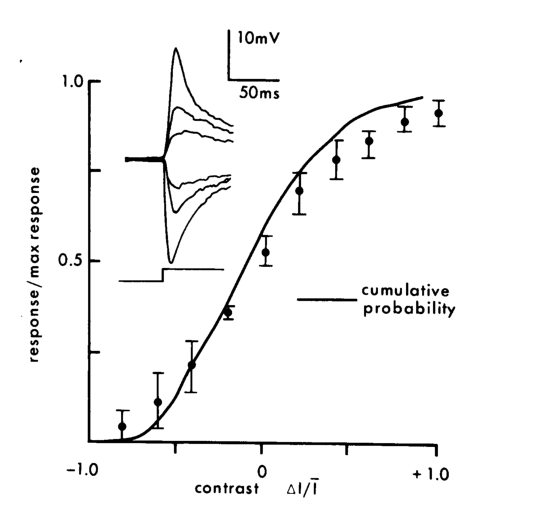
\includegraphics[width=\columnwidth]{figures/laughlin_81.eps}
\label{fig:laughlin}
\caption{The response function of the blowfly LMC closely resembles the cumulative distribution of visual contrasts in its natural environment. Figure taken from Laughlin, S. (1981)}
\end{marginfigure}

This framework can also be generalized to a population of neurons. Writing $O_i$ for the random variable associated with the output activity of each neuron and $O$ for the population activity, we can decompose the redundancy into two terms, yielding
$$
\mathcal{R} = \frac{1}{C} \left(C - \sum_i H(O_i) \right) + \frac{1}{C}\left(\sum_i H(O_i) -H(O)\right).
$$
The first term accounts for redundancy arising from unequal frequency of use of different symbols and the second accounts for redundancy arising from 
correlations between the activities $O_i$. In the example above we have only had to deal with the left term, since we had only one activity and therefore no 
correlations between them. A lot of the efficient coding literature, however, has dealt with the second term, and a number of different approaches have looked 
towards independent components of natural stimuli, assuming that whitening or gain control could account for the maximization of the first term.\par

Michael Lewicki, for example, demonstrated that using independent component analysis\footnote{Indepedent Component Analysis, or ICA for short, tries to 
decompose a signal into a set of features which are statistically independent between them. This can be done by minimization of a number of different cost 
functions.} on a set of natural sounds, comprised of human speech, animal vocalizations and natural background sounds, one recovers receptive fields similar to 
the receptive fields of early auditory neurons.\cite{Lewicki2002} There have been a number of similar studies based on different efficiency measures. 
Another way to interpret Barlow's approach is to eschew information theory and to take the hypothesis that the response of sensory systems seek to represent
in a way that allows for optimal reconstruction while minimising the number of spikes employed. This approach is often called \emph{sparse coding} since the
resulting codes will show response with sparse activity in the neural population. Bruno Olshausen and David Field,\cite{Olshausen1996} for example, have shown 
that, applying the sparse coding approach to a set of natural images results in filters similar to receptive fields in primary visual cortex.\footnote{Sparsity is in 
principle given by the number of active neurons, or if the response is graded by the sum of the activities of the neurons. This leads to cumbersome mathematics
and the kurtosis of the activity is usually employed as a surrogate for the sparsity.}\par

These results and a number of other similar studies have lent considerable traction to the idea that the nervous system is adapted to encode the stimuli present in 
the animal's natural environment. This approach, however, is not without its issues. For one, the limit of Shannon's theorem, in which the redundancy of the code is 
very small, turns the code ever harder to decode. Another important point is that, although minimizing dependence between filters yields good estimates of 
receptive fields observed in the brain, neurons' activities in the brain are far from independent.\footnote{Insert citation about correlations in brain} Though the 
redundancy reduction approach has provided numerous insights as mentioned above, other ideas have emerged since.
\par

\section{The Bayesian Brain}

The finding that humans perform near-optimally\marginnote{Optimality is used in the Bayesian sense, where we mean the subjects integrate uncertain information according to Bayes' rule} when integrating uncertain cues from different senses have led neuroscientists to theorize that the brain explicitly represents distributions over world states.\cite{Ernst2002,Ma2006} In these so-called probabilistic population codes, a spike would contribute to the computation of a posterior probability over world states with a likelihood depending on its conditional probability of firing given the stimulus. This leads to a Bayesian interpretation of the activity of the brain, where the reliability of different sensory cues can be taken in account when integrating them. It can also be argued that representing the uncertainty of events in the world has an important role in decision-making, and will therefore serve as an evolutionary advantage. To use a popular example,\footnote{This example is discussed in \citep{Ma2006}.} let us consider the case of a person deciding wether or not to jump over a stream filled with piranhas. The stream is 1.8 meters wide, and the person jumps an average distance of 2.1 meters. One will be inclined to suggest jumping.\marginnote{Should you jump over a stream filled with piranhas?} Yet both the width of the stream ($w$) as the jumping distance ($j$) are estimated based on uncertain information, and therefore could be imprecise estimates (in the case of the width) or subject to random variation (in the case of the jump distance). Suppose our best guess of the width of the stream is a normal distribution with mean 1.8 meters with a standard deviation of 0.1 meters. Furthermore suppose the standard deviation of the jump distance is 0.4 meters. That would give us a probability of approximately 0.23 of falling down the cliff. So one would definitely be less inclined to jump over the stream, or would at least take preventive actions to minimize the uncertainty in both your estimate of the width of the stream and your jump.\par
From a neural perspective, we could then infer the stimulus distribution (distribution over stream widths) given the response of a neuron population and a model of its response variability. If we assume a given neuron responds according to a certain distribution $P(r|s)$\marginnote{Here we term $r$ the response and $s$ the stimulus}, the Bayesian posterior is given simply by
\[
P(s|r) = \frac{P(r|s) P(s)}{P(r)} \propto P(r|s) P(s).
\]
Assuming independent firing for a number of neurons, whose response distributions are given by $P(r_i|s)$ we would have simply
\[
P(s|\{r_1,\ldots,r_n\}) \propto P(s) \prod_i P(r_i|s).
\]
One then still has to determine the nature of the neural variability given by $P(r|s)$. This distribution is often taken to be Poisson. This means that for very short time intervals, of duration $dt$, the probability of neuron $i$ spiking would be given by a rate function $f_i(s)$, as
\[
P_{dt}(r_i|s) \approx f_i(s) dt.
\]
The true Poisson distribution for spike counts assuming the stimulus does not change during a time interval of duration $T$ is given by\marginnote{Poisson distribution}
\[
P_T(r_i|s) = \frac{e^{-f_i(s) T}f_i(s)^{r_i}}{r_i!}
\]
The rate function $f_i(s)$ is often called the tuning function of the neuron. Given a number of neurons in primary visual cortex responding to the edges of the stream, one could then estimate the stream from those responses according to a simple model as
\[
P(width|{r_1,\ldots}) \propto P(width) \prod_i P(r_i|width),
\]
and likewise obtain the mean and standard deviation of our estimate. More simply we can look for the maximum a posteriori estimator, the value of $s$ that maximises
the probability $P(width|{r_1,\ldots})$. It is often more convenient to maximise the log-probability $\log P(width|{r_1,\ldots})$. Often an additional assumption of a flat
prior is made, yielding the Maximum likelihood estimator.
\par
Note that given a distribution over visual stimuli or a distribution over stream widths, one could seek a set of tuning functions $f_i(s)$ such that the standard deviation 
of our estimate is minimal. This is clearly a very broad formulation of the problem, but it will be the central question studied in this thesis. Alternatively, one could look
directly at the (expected) cost associated with a decision (to jump or not to jump) and choose the set of functions $f_i(s)$ which minimises the future expected cost.
We will investigate the difference between these approaches as well.
\par

Why would an organism be interested in estimating the distribution of world states conditioned on the activity of its sensory systems, though? For one, there is
the finding that the best estimator for the world's state is the mean of the posterior distribution (see \fref{chap:mse}). This means that regardless of the particulars
of the response properties of the sensory system, the posterior mean gives us the world's estimate with the lowest expected quadratic error. A second important
reason is multisensorial cue integration. Let us assume we have a visual and an auditory cue for the width of said stream.\footnote{A foggy view of the opposite 
margin ($v$) and a faint voice talking from the opposite margin ($a$).} Both lead us to different estimates of the stream's width ($\hat{w}_v$ for the visual estimate 
and $\hat{w}_a$ for the auditory estimate). There are countless ways of combining these two to obtain a final estimate of the width. But without further information
on the posterior distributions $P(w|a)$ and $P(w|v)$ we have no way of knowing the best way to combine them. If we had knowledge of them, we could simply
evaluate the full posterior mean\footnote{Assuming the auditory and visual stimuli are uncorrelated conditioned on the world's state.}
\[
\hat{w}_{a,v} = \int dw w P(w|a,v) = \int dw w \frac{P(a|w)P(v|w)P(w)}{P(a)P(v)}.
\]
In the case of Gaussian distributions, we would have $P(w|a) = \mathcal{N}(\hat{w}_a,\sigma_a)$, and $P(w|v) = \mathcal{N}(\hat{w}_v,\sigma_v)$, leading to the simple
cue integration rule
\[
\hat{w}_{a,v} = \frac{\sigma_v \hat{w}_a + \sigma_a \hat{w}_v}{\sigma_a + \sigma_v},
\]
There is no simple formula like this in general, though, leading to the need to estimate the full distribution.
\par


%
%\section{Dynamic Population Coding}
%
%We have had to assume that the stimulus did not change during the response of the neurons to evaluate the Poisson probability of a number of spikes being fired by a neuron. If we relax this assumption, and assume now that the stimulus evolves during time, being now a dynamic stimulus $s(t)$, we will have to reformulate the neural variability model. The probability for infinitesimal time intervals remains the same though. If we denote the number of spikes fired by neuron $i$ since the beginning of the experiment by $N_i(t)$, we can write then
%\[
%P(N_i(t+dt) - N_i(t) = 1|s(t)) = f_i\left(s(t)\right) dt,
%\]
%and 
%\[
%P(N_i(t+dt) - N_i(t) = 0|s(t)) = (1-f_i\left(s(t)\right)) dt.
%\]
%Denoting the limit with $dt\to 0$ of the difference as $dN_i(t)$, we can write the probability of a spike train given by $N_i = \{N_i(\tau), \tau \in [0,T]\}$ conditioned on the stimulus history $s = \{s(\tau), \tau \in [0,T]\}$ as
%\[
%P(N_i|s) = \exp\left(-\int_0^T f_i(s(\tau)) d\tau + \int_0^T \log\left[f_i(s(\tau))\right] dN_i(\tau) \right)/N_i(T)!.
%\]
%We are using the notation of stochastic calculus, where the stochastic integral over a jump process is given by
%\[
%\int f(t) dN(t) = \sum_{t_i} f(t_i) (N(t_i) - N(t_i^-)),
%\]
%where $N(t_i^-) = \lim_{t\uparrow t_i} N(t)$. This can be made rigorous in the language of Martingales but we will keep the discussion simple, as most of the processes
%considered are well behaved Poisson or Wiener processes.
%In that sense we can estimate the probability of the entire stimulus history given a spiking history of a population of neurons as
%\[
%P(s|\{N_1,\ldots,N_n\}) = P(s) \prod_i P(N_i|s),
%\]
%furthermore we can marginalize out all but the present value of $s$ to obtain the filtering probability
%\begin{equation}
%\label{eq:filtering_eq_path}
%P(s(T)|\{N_1,\ldots,N_n\}) = \int d\mu(s\setminus T) P(s) \prod_i P(N_i|s),
%\end{equation}
%where $d\mu(s\setminus T)$ denotes the measure over all paths of the stimulus $s$ ending at the given value of $s(T)$. In all but a few exceptions, we will focus in
%this thesis on the Gaussian measure over paths defined by a Gaussian process. A Gaussian process is a random variable $g$ such that for any set of points in its
%domain $\{t_1, t_2, \ldots , t_N\}$, the distribution of $\{g(t_1), g(t_2), \ldots, g(t_N)\}$ is Gaussian with mean $\{\mu(t_1),\mu(t_2),\ldots,\mu(t_N)\}$ and covariance
%matrix $\left<\left(g(t_i) - \mu(t_i)\right)\left(g(t_j)-\mu(t_j)\right)\right> = K(t_i,t_j)$. $K(u,v)$ is commonly called the Kernel of the Gaussian process. Gaussian 
%Processes, or GP's have been extensively used for numerical regression, smoothing, classification and other uses in machine learning and signal 
%processing \cite{Rasmussen2005}. Simple examples of Gaussian processes are the Wiener process, the Ornstein-Uhlenbeck process and the Radial-Basis-Function
%processes. Gaussian Processes allow for a number of simplifications in practice, and in the case we consider, the posterior distribution can be computed exactly.\par
%In practice, we now need to compute averages of the Poisson likelihood over paths of a Gaussian process. This is general very complicated, and approximations are
%usually employed to decode the stimulus from the spike train.\cite{Ahmadian2011,Ergun2007} Looking at \fref{eq:filtering_eq_path} for the Poisson case we can write
%\begin{align*}
%P(s(T)|\{N_1,\ldots,N_n\}) \propto& \int d\mu(s\setminus T) P(s)\\
%& \exp\left(-\sum_i \int_0^T f_i(s(\tau)) d\tau + \sum_i \sum{t_i} \log\left[f_i(s(t_i))\right]  \right).
%\end{align*}
%There are two terms in the exponent, one referent to the actual occurrence of spikes at the spike times, and one accounting for the absence of spikes in all other 
%instants. If we only had to deal with the actual spike times, the task of inferring the posterior is substantially simpler, as we could perform approximate inference
%over a finite set of points, instead of evaluating averages over all possible paths. This would be the case if the sum of the rates over all neurons was constant, or
%at least independent of the value of the stimulus $s(t)$. This is the dense coding regime, as a dense packing of the tuning curves over the space of the stimulus
%$s$ will lead to a population firing rate which is insensitive to $s$. In that case we would have $\sum_i f_i(s(t)) = C$, and the posterior can be further simplified to
%\[
%P(s(T)|\{N_1,\ldots,N_n\}) \propto \int d\mu(s\setminus T) P(s) \prod_i \prod_{t_i} f_i(t_i).
%\]
%This is often also used as an approximate inference procedure, as accounting for the absence of spikes throughout the duration of the experiments often makes the
%inference problem much harder. We will further simplify the problem by assuming that the tuning functions $f_i$ are unnormalised Gaussians, turning the problem of
%evaluating the posterior into a Gaussian Process Regression problem. This will allow us to treat the evolution of the MSE of the optimal Bayesian estimate for a
%given population of neurons using the language of statistical physics. This had been done similarly for the case of Gaussian Process regression in the smoothing
%case,\cite{malzahn2005statistical} but to the author's best knowledge it had not been studied for the filtering case before. This has allowed us to obtain a number of
%analytic results. The general case, however, must be dealt with numerically, and we review a few techniques for the filtering of stochastic processes under
%general conditions.\par



%The main goal of neuroscience is to answer a simple yet puzzling question: {\em What is the brain doing?} One might argue that we know a lot about what the brain is doing, at least on the phenomenological side, yet the more conceptual levels of what problem the brain is solving, or what it is good at doing, are far from answered. The main analogy we see in use in the field of neuroscience is that of the brain as a computer, hence the frequent use of concepts from Shannon's mathematical theory of communication. Namely, it is frequently hypothesized that the brain is optimally representing interesting aspects of the world it perceives. This thesis seeks to discuss the concept of optimal coding in neural systems. In it, I will discuss mainly findings in filtering of stochastic processes from point process observations and its relation to optimal population coding.\par
%Filtering is of general interest because of its relation to optimal control. More precisely, when considering a linear quadratic control problem under Gaussian noise conditions, the {\em separation principle} holds, and we can design an optimal controller by first predicting the state of the system, and then choosing the optimal control for the noiseless case on that state. The prediction step is solved by the Kalman filter. This framework is frequently used in the study of motor control, and a number of recent experiments and developments have relied on optimal control theory to model the properties of animal subjects under specific noise conditions. Here I will argue that the same approach should also be considered in the sensory areas of the brain.\par
%Investigators have repeatedly hypothesized that the shape of receptive fields and the response properties of sensory neurons can be traced back to optimality with respect to some criterion. The first approach, which drew heavily from Shannon's information theory, was Barlow's efficient coding hypothesis. In its initial form, it stated that the code employed in sensory systems should be adapted to the stimulus distribution in a way to minimized the redundancy, as defined in information theory as the difference between the code capacity and the source entropy divided by the code capacity. Many different efficiency measures have since been proposed. Metabolical considerations favor the use of sparse codes, where at any given time only a few neurons are active.\par
%Another popular approach is to use the Cramer-Rao bound of statistics, and maximize the fisher information of the code, so minimizing a lower bound on the mean-squared-error of the estimator. This has been very popular and is still widely employed in the theoretical neuroscience literature. This bound, however, has been proven to not be tight in useful regimes, and more recently a shift towards using the minimum of the mean-squared-error directly as an efficiency measure has been taking place. We focus here on this measure of efficiency, which we will motivate through optimal control theory in chapter ?? (INSERT REFERENCE).\par
%An alternative approach, which is still in its budding phase, is to consider directly optimal control problems and from the average cost incurred by a given code, choose an optimal code for a given task. This is hindered by the considerable analytical problems involved in treating optimal control problems analytically. I will show, however, that in the popular framework of dense Gaussian tuning functions, an exact expression can be found for the optimal cost-to-go of a linear-quadratic-Gaussian control problem. This bypasses the somewhat abstract notion of an efficiency criterion to consider directly the costs of a given code to the animal using it. It does so at the considerable expense of oversimplifying the problems faced by an animal to an impressive amount. Yet, the approach considers the problem of optimal coding from a more holistic perspective, considering representation and coding as a cog in a machine rather than and end in itself.\par
%
%\section{Structure}
%
%I will start out by reviewing the literature and the different approaches to optimal population coding in chapter ??, giving special attention to the case of mean-squared-error minimization which is considered in this thesis. In the following chapter, I briefly introduce the theory of filtering of point-process observed stochastic processes. Here, the general theory of filtering is presented and the simplifications introduced by the dense Gaussian tuning function limit are discussed. In the following chapter, I discuss results on the mean-squared-error in filtering of Gaussian processes, providing analytical results and comparing it to simulations. The derivations are also compared with a replica-type approach which yields the same results. In the following chapter I consider the problem of optimal control using point-process observations. This is discussed briefly, and a derivation for the optimal cost-to-go is presented. Finally, I consider the implications of the approaches developed to a ecological theory of sensory processing. Namely, I consider the relationship between optimal tuning widths and firing rates with the timescales and correlation lengths in the processes. This is also done numerically for a number of cases that are analytically intractable. I finalize by discussing the presented research, its impact and relation to previous research and future directions of research.
%\cite{susemihl2011}

%We will argue that filtering of stochastic processes is a good proxy for the neural representation of stimuli in the brain.\par

%This presents a number of problems, which we will address in this thesis.

\chapter{Filtering and Prediction with Point Process Observations}

\label{chap:filtering}

\section{Fast Population Coding}

\section{General Filtering for Point Process Observations}


\section{Offline Inference}

\section{Prediction}

\chapter{Mean-Squared-Error for Point Process Filtering}

\label{chap:MSE}

\chapter{Optimal Control with Point Process Observations}

\label{chap:control}

\newthought{Clearly the nervous system is not solely interested in estimating the state of the world.} Furthermore, if that estimate is not useful for making decisions and taking actions 
in a dynamic environment, there is little use for it. In the previous chapter I have discussed findings for spiking codes in an estimation context. In this chapter I will extend this approach 
to the framework of stochastic optimal control, and discuss how to reframe the findings in this context.\par

The field of optimal control has been of growing interest to the neuroscience community, but little attention has been given to the issue of optimal coding in a control context. Here I
will study a simple case of linear quadratic control observed through a dense population of Gauss-Poisson neurons, for which I have been able to derive a closed-form expression
for the optimal cost-to-go. This allows one to study the expected control cost in an experiment as a function of the encoder, similarly to what I have done with the MMSE in the previous 
chapters. Furthermore, in \fref{chap:optimal} I will compare these two approaches, showing that in a couple of simple examples, the control-optimal and the MMSE-optimal encoders
differ significantly.

\section{Optimal Control}
The field of control theory is concerned with the steering and controlling of systems, always with the minimization of a cost (or maximization of a reward) in mind. Speaking mathematically, given a system with state $X(t) \in \mathcal{X}$, with dynamics given by
$$
\dot{X}(t) = f(X(t),U(t)), \quad X(0) = x_0
$$
one would like to select the control variables $U(t) \in \mathcal{U}$ in such a way as to minimize an integrated cost function over time\footnote{This is an additive cost function,
which is itself only a specific kind of control problem. Generally one can also consider more complex cost functions as well, that depend on the minimum or maximum
of the state or multiplicative cost functions.}
$$
C(X_{0:T},U_{0:T}) = \int_{0}^T c(X(s),U(s),s) ds + h(X(T)).
$$
Here $c(x,u,t)$ specifies a cost rate accumulated over time and $h(x)$ describes some final goal the system should achieve at the end of the control problem.\par

In a purely deterministic setting, the solution to the control problem would be a policy $U^* : \mathcal{X} \times \mathbf{R}\to \mathcal{U}$ which for each system 
state and time gives a control to be applied to the system when it is in that state at that time. One would have\marginnote{The minimum of the future cost over the space of controls is called the value function $V(X,t)$.}
$$
\min_{U_{0:T}} C(X_{0:t},U_{0:t},0;x_0) = C\left(X_{0:t},U^*(X_{0:t}),0\right) \equiv V(x_0,0),
$$
where $V(x,t)$ is usually called the optimal cost-to-go function or the value function. $V(x,t)$ quantifies the cost one is expected to incur if he controls the system optimally through the 
remainder of the control problem, given that the system is at state $X(t)=x$ at time $t$.\par

This is a very broad formulation, but one general remark can be made, though, first put forward by Richard Bellman.\mycite{Bellman1952} Bellman 
proposed an optimality principle\marginnote{Bellman's principle of optimality}, which stated that if a given policy is an optimal solution to a control problem, then the 
policy resulting after a number of steps of that policy must still be optimal for the remaining control problem as well. This can be formulated as a mathematical equation, 
the so-called Bellman equation or dynamic programming equation, which states that the minimal future cost in state $X(t)$ at time $t$ is given by the minimum over 
$U(t)$ of the instantaneous cost plus the minimal future cost at the resulting future state $X({t+dt})$. Mathematically, we have
\begin{equation}
\label{eq:bellman_eq}
V(X(t),t) = \min_{U(t)} \left[ c(X(t),U(t),t) dt +V(X({t+dt}),t+dt)\right].
\end{equation}
Note that in general, $X({t+dt})$ will depend on $U(t)$, making the solution of the Bellman equation difficult.\par
In continuous time, assuming differentiability of the value function $V$ in both its, one obtains
\[
V(X(t),t) = \min_{U(t)} \left[c(X(t),U(t),t) dt + V(X(t),t) + \frac{\partial V}{\partial t} dt + \frac{\partial V}{\partial x} dX(t) \right],
\]
which leads to the Hamilton-Jacobi-Bellman equation\marginnote{I will abbreviate the Hamilton-Jacobi-Bellman equation as HJB equation.}
$$
-\frac{\partial V}{\partial t} = \min_{U(t)} \left[c(x,U(t),t) + \frac{\partial V}{\partial X} f(x,U(t)) \right].
$$
This is often more convenient to solve, as it sometimes allows for explicit minimisation over the control. The HJB equation must be solved backwards in time, with final condition $V(x,T) = h(x)$.

\subsection{Estimation and the Separation Principle}

In the previous two chapters, I have considered the problem of filtering a stochastic process from spike trains. More specifically, given a signal, I was looking for the optimal set of 
parameters $\varphi^*$ for a population of neurons that minimise the MMSE of the filtering problem. Here I would like to establish a similar approach to control problems. That is,
in the same sense of before, I have a noisy system observed through spike trains of a population of neurons specified by some parameters $\varphi$, but now I am concerned with
controlling this noisy system. Given a cost function, I would like to determine the parameters $\varphi^*$ that minimise the control costs, instead of the filtering error.
If one is interested in controlling a system, say a limb performing a movement, one must now deal with the uncertainties in the system and control it according to noisy estimates of its 
state. The certainty equivalence property (CEP) holds if a system one only has partial information about can be controlled ignoring the uncertainty in its state and acting as if it were 
fully observed. I will elaborate below.
\par

Consider a deterministic system
\[
\dot{X} = f(X(t),U(t)),
\]
where I have only partial knowledge about the system's state through an initial distribution $P_0(x)$ and noisy observations $Y(t)$ of the system's state. If the certainty 
equivalence property holds for this system, the optimal control for the partially-observed system, will be the optimal policy of the fully observed problem applied to the mean estimate
of the system's state. To be more precise, let me define the cost for the partially-observed system as
\[
C(P_0,Y_{0:T},U,0) = \int_0^T \boldsymbol{E}  \left[c(X(s),U(s),s) \mid Y_{0:s},P_0 \right]ds + \boldsymbol{E} \left[h(X(T))\mid Y_{0:T},P_0\right].
\]
The optimal control $U^*$ will now be a function of the observations $Y_{0:t}$ up to time $t$ and the initial distribution $P_0$. If the optimal control for the fully-observed system is 
given by $U^*_{obs}(x,t)$, the certainty equivalence property holds if the optimal control for the partially observable process is given by 
$$
U^*_{part} (Y_{0:t},P_0,t) =  U^*_{obs}\left(\boldsymbol{E}\left[X(t) \mid Y_{0:t},P_0\right],t\right).
$$
This means that the uncertainty in the system's state can be treated in two independent steps, first estimating the system's state through the posterior mean and then applying the
control as if our estimate of the state was certain. Hence the name certainty equivalence, as one applies the control as if they were certain about the system's state.
The separation property is also frequently discussed in the literature, and it is a stronger version of the certainty equivalence property, where the control $U^*_{obs}(x,t)$ being 
employed does not need
to be the optimal policy for the fully observed problem, but can be related to some other control problem with full informations.\par

One can now ask what is the encoder that minimises the expected control costs. It is tempting to conclude from the CEP that the encoder that minimises the MMSE also minimises
the control costs. This is not true, however, as I will show in \fref{chap:optimal}. I will now consider the case of stochastic optimal control, and then turn to the case of 
partially-observable stochastic optimal control. This can be treated for the case of dense Gauss-Poisson observations, and I will derive a novel relation for the optimal cost-to-go
for that case.

\section{Stochastic Optimal Control}

The world is a noisy place, and if to control real-world systems, one must be able to account for noise in the systems as well. One simple way to include noise is to generalise the system dynamics to a stochastic differential equation. Consider
$$
dX(t) = f(X(t),U(t)) dt + H^{1/2} dW(t),
$$
where $W(t)$ is a standard Wiener process. It is not possible to predict the evolution of $X(t)$ exactly anymore, so one must redefine the cost function. The natural way
to do so is to define it as the average over future states conditioned on the current state $X(t)$ and the controls to be applied $U(t)$. This will lead to
\[
C(X,U) = \boldsymbol{E} \left[\int_0^T c(X(t),U(t),t) dt \biggm\vert X(0), U_{0:T}\right].
\]
One should mention that there are other ways to deal with the stochastic nature of the problem, such as the risk-sensitive control approach,\mycite{whittle1981} where one considers
the cost function
\[
C_{\theta}(X,U) = \frac{1}{\theta} \log \boldsymbol{E} \left[\exp\left(-\theta \left(\int_0^T c(X(t),U(t),t) dt + h(X(T))\right)\right)\right].
\]
In the limit $\theta\to 0$ one recovers the former formalism. This allows one to consider risk-averse or risk-seeking control policies. I will not, however, consider this approach here.\par
The Bellman equation can then be extended to the stochastic case as
\begin{equation}
\label{eq:stochastic_bellman}
V(x,t) = \min_{U(t)}\boldsymbol{E}\left[ c\left(X(t),U(t),t\right) dt + V\left(X(t+dt),t+dt\right)\mid\,X(t)=x, U_{[t,T]}\right].
\end{equation}
Using It\=o's lemma for the variation of $V$, and averaging over the Brownian motion $dW(t)$ leads to
\[
V(x,t) = \min_{U(t)} \left[ c(x,U(t),t) dt + V\left(x,t\right)+\left(\frac{\partial V}{\partial t} dt + f(x,U(t))^\top \frac{\partial V}{\partial x} +\frac{1}{2} \Tr\left[H \frac{\partial^2 V}{\partial x^2} \right]\right)dt \right].
\]
This leads to the stochastic HJB equation
\begin{equation}
\label{eq:stochastic_HJB}
-\frac{\partial V}{\partial t} = \frac{1}{2} \Tr\left[H \frac{\partial^2 V}{\partial x^2} \right] +\min_{u} \left[ c(x,u,t)  + f(x,u)^\top \frac{\partial V}{\partial x}\right].
\end{equation}
\par
One could also consider a Poisson process as a noise source. If one takes, for example, a Poisson counting process $N(t)$, with time- and/or
 state-dependent rate $\lambda(X(t),t)$, and takes the system dynamics to be given by a drift-diffusion process with state-dependent jumps $j(X(t),t)$, occurring with
 rate $\lambda(X(t),t)$ then the SDE for the state would be,
$$
dX(t) = f(X(t),U(t)) dt + H^{1/2} dW(t) + j(X(t),t) dN(t).
$$
This would lead to the full HJB equation for a drift-jump-diffusion process controlled by some control process $U(t)$
\begin{equation}
\label{eq:martingale_HJB}
-\frac{\partial V}{\partial t} = \min_{u} \left[c(x,u,t) + f(x,u)^\top \frac{\partial V}{\partial x} + \frac{1}{2} \Tr\left[H \frac{\partial^2 V}{\partial x^2} \right] + \lambda(x,t) \left[V(x+j(x,t),t)-V(x,t)\right]\right],
\end{equation}
now including the terms regarding the jump process.\mycite{Theodorou2012,Sennewald2006} Note that the statistics of the posterior distribution of the filtering problem from the previous
chapters fit this description, namely they are a jump-drift processes with no diffusion. I will use this formalism to derive a belief state formulation of a control problem with dense
Gauss-Poisson observations.

\subsection{Linear-Quadratic-Gaussian Control}

The Linear-Quadratic-Gaussian\footnote{LQG} control problem is defined by linear dynamics in both the state and the control variable, a quadratic cost rate function
$c$ in both the state and control and a Gaussian noise source. I will treat this problem here to illustrate the optimal control formalism.
This would mean that the evolution of the state is given by the SDE
\begin{equation}
\label{eq:ctl_diff_dyn}
dX(t) = \left(A X(t) + B U(t)\right) dt + H^{1/2} dW(t),
\end{equation}
where $W(t)$ is a Wiener process. Taking a cost rate given by
$$
c(X(t),U(t),t) = U(t)^\top R(t) U(t)+ X(t)^\top Q(t) X(t),
$$
and a final cost given by $h(X(T)) = X(T)^\top Q_T X(T)$, one can solve for the value function explicitly, using the HJB equation. The HJB equation in this case will be given by
$$
-\frac{\partial V}{\partial t} = \min_{U(t)} \left[ U(t)^\top R(t) U(t) +  x^\top Q(t) x + \frac{\partial V}{\partial x}^\top \left(A x  + B U(t)\right) + \frac{1}{2} \Tr\left(H\frac{\partial^2 V}{\partial x^2}\right) \right].
$$
One can minimize the right hand side explicitly and eliminate $U$ from the equation. One obtains that the optimal control is given by
$$
U^*(x,t) = -\frac{1}{2} R(t)^{-1} B^\top\frac{\partial V}{\partial x}\big|_{x,t}.
$$
Inserting into the HJB equation once more leads to
\begin{equation}
\label{eq:lqg_hjb}
-\frac{\partial V}{\partial t} = x^\top Q(t) x +\frac{\partial V}{\partial x}^\top A x -\frac{\partial V}{\partial x}^\top B R(t)^{-1} B^\top \frac{\partial V}{\partial x} + \frac{1}{2}\Tr\left(H\frac{\partial^2 V}{\partial x^2}\right).
\end{equation}
It can be shown that $V$ can only have a quadratic dependence in $X$, since at the final time the cost is given by $h(X(N))$ which is quadratic, and the HJB equation will preserve
this property. I will assume it is of the form $V(x,t) = x^\top S(t) x + \alpha(t)^\top x + k(t)$. Inserting this into \fref{eq:lqg_hjb}
gives the ODE's for the parameters of the value function
$$
-\dot{S} = Q(t) + A^\top S(t) + S(t) A - S(t) B R(t)^{-1} B S(t),
$$
$$
-\dot{\alpha} = A^\top \alpha(t)-S(t) B R(t)^{-1} B^\top \alpha(t),
$$
$$
-\dot{k} = \Tr\left(H S(t)\right)-\alpha(t)^\top B R(t)^{-1} B^\top \alpha(t),
$$
with the terminal conditions $S(T) = Q_T$, $\alpha(T) = 0$ and $k(T)=0$. The $X$-independent term $k(t)$ accounts for the future uncertainty in $X$, decreasing to $0$ over time as we approach the final time $T$. Furthermore, the differential equation for $S(t)$ is a special case of the Riccati equation. The full optimal control for the LQG control problem will 
therefore be given by
\[
U^*(x,t) = -R(t)^{-1}B^\top S(t) x.
\]

These results can also be extended to the case of control- and state-dependent diffusion noise, affine dynamics and some other cases.\mycite{Kappen2011}

\section{Partially Observable Processes}

In general, one does not have access to the exact state of the system, and it is useful to consider cases where one is only given noisy observations of the state, as were considered in 
the previous chapters. The most commonly considered case of partially observable control problem is a LQG problem observed through a second diffusion process. Suppose one has 
as above a system $X(t)$ evolving according to \fref{eq:ctl_diff_dyn}, but instead of observing $X(t)$ directly, one observes the process $Y(t)$, which I shall call the 
observation process, given by
\begin{equation}
\label{eqn:ctl_obs_dyn}
dY(t) = C X(t) dt + D^{1/2} dV(t).
\end{equation}
Given a control trajectory $\{U(s), s\in [0,t]\}$, the problem of estimating $X(t)$ given observations ${Y(s), s \in [0,t]}$, is a simple filtering problem, and is solved exactly by the Kalman-Bucy filter.\footnote{See \fref{chap:filtering}.} It will lead to a Gaussian estimate of $X(t)$ with mean $\mu(t)$ and variance $\Sigma(t)$, where $\mu$ and $\Sigma$ evolve according to
\begin{subequations}
\label{eq:ctl_kalman_bucy}
\begin{equation}
d\mu(t) = (A \mu(t) + B U(t))dt + \Sigma(t) C^t D^{-1} \left(dY(t) - C\mu(t) dt\right),
\label{eq:ctl_kalman_bucy_mean}
\end{equation}
and
\begin{equation}
\label{eq:ctl_kalman_bucy_var}
\frac{d\Sigma}{dt} = A \Sigma + \Sigma A^\top + H - \Sigma C^\top D^{-1} C \Sigma.
\end{equation}
\end{subequations}
Since in this case we do not have perfect information on the process to be controlled, we have to settle for the goal of minimizing the expected cost given our observation. Therefore, the cost to be minimized is
$$
C(U_{0:T};\mu_0,\Sigma_0) = \boldsymbol{E}\left[\int_{t_0}^T c(X(t),U(t),t)dt +h(X(t))\right],
$$
where the average is over all future paths of $X(t)$ and all observation paths $Y(t)$.
There is no analogous to the HJB equation for the incomplete information case, but I will reformulate the problem as a control problem over the belief states, that is, the state of the world as one is led to believe it is distributed given the previous observations\marginnote{The belief state is a description of an system with incomplete information which eschews describing the actual state of the system, instead describing the distribution over states. A general formulation is described in \mycitep{bertsekas2012}.}. In the case I am discussing, the belief state is the distribution over the state variable, given by the Gaussian distribution $\mathcal{N}(\mu(t),\Sigma(t))$. The dynamics of the belief state is then given by equations \fref{eq:ctl_kalman_bucy_mean} and \fref{eq:ctl_kalman_bucy_var}. Note that when one chooses to describe the system in terms of the mean and variance of the posterior distribution, the noise process $dW(t)$ does not enter into the analysis anymore, and the observation process $dY(t)$ takes the role of the noise process. We need, however, to redefine the cost function $c(X(t),U(t),t)$ to fully specify the problem. The average cost is
$$
\boldsymbol{E}\left[c(X(t),U(t),t)\middle|\mu(t),\Sigma(t) \right] = U(t)^\top R(t) U(t) +\left(\mu(t)^\top Q(t) \mu(t) + \Tr\left(Q(t)\Sigma(t)\right)\right),
$$
from which one can define a belief-state cost rate, which makes no mention of the underlying unobservable process
\[
c(\mu,\Sigma,U,t) =  U(t)^\top R(t) U(t) +\mu(t)^\top Q(t) \mu(t) + \Tr\left(Q(t)\Sigma(t)\right).
\]
One can now write the HJB equation for the system described by \fref{eq:ctl_kalman_bucy}, leading to
$$
V(\mu(t),\Sigma(t),t) = \min_{U(t)} \boldsymbol{E}\left[ U(t)^\top R(t) U(t)+\left(\mu(t)^\top Q(t) \mu(t) + \Tr\left(Q(t)\Sigma(t)\right)\right)+V(\mu(t+dt),\Sigma(t+dt),t+dt)\right],
$$
where the expectation is now with respect to the observation process $Y(t)$.
Taking the variation of $V$ with infinitesimal time increments via It\=o's lemma one has
$$
dV = \frac{\partial V}{\partial t} dt + \frac{\partial V}{\partial \mu}^\top d\mu + \Tr\left[\frac{\partial V}{\partial \Sigma}d\Sigma\right] +\frac{1}{2} \Tr\left[(\Sigma C^\top D^{-1} C 
\Sigma)_{i,j} \frac{\partial^2 V}{\partial \mu^2}\right],
$$
which leads to the HJB equation
\begin{eqnarray*}
-\pd{V}{t} =& \min_{U(t)} \boldsymbol{E}\left[ U(t)^\top R(t) U(t)+\mu(t)^\top Q(t) \mu(t) + \Tr\left(Q(t)\Sigma(t)\right) +\frac{\partial V}{\partial \mu}d\mu^\top\right] \\&+ \Tr\left[\frac{\partial V}{\partial \Sigma}d\Sigma\right] +\frac{1}{2} \Tr\left[(\Sigma C^\top D^{-1} C \Sigma)_{i,j} \frac{\partial^2 V}{\partial \mu^2}\right] .
\end{eqnarray*}
Minimization with respect to $U(t)$ leads to $U^*(t) = -R(t)^{-1} B^\top \pd{V}{\mu}$, which results in
\begin{eqnarray}
-\pd{V}{t} =& \mu^\top Q(t)\mu + \pd{V}{\mu}^\top B R(t) B^\top \pd{V}{\mu} + \Tr\left(Q(t)\Sigma(t)\right) +\frac{\partial V}{\partial \mu}d\mu^\top\nonumber\\&+ \Tr\left[\frac{\partial V}{\partial \Sigma}d\Sigma\right] +\frac{1}{2} \Tr\left[(\Sigma C^\top D^{-1} C \Sigma)_{i,j} \frac{\partial^2 V}{\partial \mu^2}\right] .
\label{eq:lqg_hjb_partial}
\end{eqnarray}
This would now have to be solved backwards from $V(\mu,\Sigma,T) = \mu^\top Q_T \mu + \Tr[\Sigma Q_T]$. \Fref{eq:lqg_hjb_partial} provides a clean formulation of the control problem in 
terms of the belief state, where the underlying process has been integrated over completely. This is a very useful approach and I will leverage it for the case of Point processes
observations below.
If I write the value function as $V(\mu,\Sigma,t) = \mu^\top S(t) \mu + f(\Sigma,t)$, I will obtain the same Riccati equation for $S(t)$ as in the fully observed case. Using this form for
the value function, one immediately recovers the optimal control $U^*(t) = -R^{-1}(t) B^\top S(t) \mu$, which shows the certainty equivalence property for this system.
\section{Partially Observable Processes with Poisson Observations}

Similarly to the case just discussed, we can consider the case of a stochastic system observed through a population of densely tuned Poisson processes with Gaussian tuning functions. The dynamics of the system would be the same as \fref{eq:ctl_diff_dyn}, but the observation processes would be given by a set of $M$ Poisson processes $N^m$ with rates given by
\begin{equation}
\label{eq:ctl_poisson_rate}
\lambda^m(X(t)) = \lambda \exp\left[-\frac{1}{2}(\theta_m-X(t))^\top \covar^\dagger (\theta_m-X(t))\right],
\end{equation}
where the tuning centres $\theta_m$ are positioned in such a way that the overall firing rate of the population $\hat{\lambda} = \sum_m \lambda^m(X(t))$ is independent of the system's
state $X(t)$.
As we have shown in \fref{chap:filtering}, the estimation problem is solved by the point-process analog of the Kalman-Bucy filter, first derived by Donald Snyder.\mycite{Snyder1972,Bobrowski2009} In the present case, with Gaussian tuning functions, the filtering equations are
\begin{subequations}
\begin{eqnarray}
d\mu(t) =& (A\mu(t) + B X(t)) dt \nonumber\\
+& \sum_i  \left[\Sigma(t^-)\left(I+\covar^\dagger \Sigma(t^-)\right)^{-1} \covar^\dagger\left(\theta_i - \mu(t^-)\right)\right]dN^i(t)\nonumber\\ 
\label{eq:ctl_poisson_mean}
\end{eqnarray}
and
\begin{eqnarray}
d\Sigma(t) =&\left(A\Sigma(t) + \Sigma(t) A^\top + H\right)dt\nonumber \\
-&  \left[\Sigma(t^-) \covar^\dagger \Sigma(t^-) \left(I+\covar^\dagger \Sigma(t^-)\right)^{-1}\right] dN(t),
\label{eq:ctl_poisson_var}
\end{eqnarray}
\end{subequations}

where $dN(t) = \sum_m dN^m(t)$. I will define 
$$
\delta \mu(t) \equiv (A\mu(t) + B X(t)) dt
$$
as the continuous part of $d\mu(t)$ and 
$$
\Delta^i \mu(t) \equiv dN^i(t) \left[\Sigma(t^-)\left(I+\covar^\dagger \Sigma(t^-)\right)^{-1} \covar^\dagger\left(\theta_i - \mu(t^-)\right)\right]
$$
as the jump part of $d\mu(t)$. Likewise, for the variance, define
$$
\delta\Sigma(t) \equiv (A\Sigma(t) + \Sigma(t) A^\top + H)dt
$$ 
and
$$
\Delta\Sigma(t) \equiv dN(t) \left[\Sigma(t^-) \covar^\dagger \Sigma(t^-) \left(I+\covar^\dagger \Sigma(t^-)\right)^{-1}\right].
$$\par
These give the evolution of the optimal Bayesian filter, with the posterior distribution over $X(t)$ conditioned on the observations $\{N^m(s), m\in [1,\ldots,M], s\in[t_0,t]\}$,
given by the normal distribution $\mathcal{N}(X(t);\mu(t),\Sigma(t))$. Assuming one is trying to minimize a cost given by the same cost rate $c(X(t),U(t),t)$ as before, one canwrite out 
the infinitesimal Bellman equation for this case as well. Since the dynamics of the system and the observations is Markov, I can use the posterior distribution as a sufficient statistic for 
the knowledge of the system's state. I will therefore take the belief state to be the mean and variance of the posterior distribution as before.\footnote{See \mycitep{bertsekas2012} for a 
more  detailed discussion.}
Similarly to the previous sections, I will consider the processes $N^m(s), s\le t$ as noise to be averaged over in the future. This leads to
$$
V(\mu(t),\Sigma(t),t)= \min_{U(t)} \left\{\boldsymbol{E}_{X(t)}\left[c(X(t),U(t),t)\right] + \boldsymbol{E}_{\{N^m(t)\}}\left[V(\mu({t+dt}),\Sigma(t+dt),t+dt)\right]\right\}
$$
According to It\=o's lemma, one obtains
\begin{eqnarray*}
V(\mu({t+dt}),\Sigma(t+dt),t+dt) =& V(\mu(t),\Sigma(t),t) + \frac{\partial V}{\partial t}dt + \frac{\partial V}{\partial \mu} \delta\mu(t) +\Tr\left[\frac{\partial V}{\partial \Sigma} \delta \Sigma(t)\right]\\ &+ \sum_m dN^m(t)\left[V\left(\mu(t) +\Delta^m\mu(t) , \Sigma(t)+\Delta\Sigma(t),t\right)-V(\mu(t),\Sigma(t),t)\right].
\end{eqnarray*}
The expectation over the noise process $N^m(t)$ in the Bellman equation can then be written as
\begin{eqnarray*}
\boldsymbol{E}(V_{t+dt})_{N^m(t)} =&V(t) + \frac{\partial V}{\partial t}dt + \frac{\partial V}{\partial \mu} \delta\mu(t) +\Tr\left[\frac{\partial V}{\partial \Sigma} \delta \Sigma(t)\right]\\ +& \sum_m \boldsymbol{E}_{N^m(t)}\left[dN^m(t)\left[V\left(\mu(t) +\Delta^m\mu(t) , \Sigma(t)+\Delta\Sigma(t),t\right)-V(\mu(t),\Sigma(t),t)\right]\right] \\
 =&V(t) + \frac{\partial V}{\partial t}dt + \frac{\partial V}{\partial \mu}^\top \delta\mu(t) +\Tr\left[\frac{\partial V}{\partial \Sigma} \delta \Sigma\right]\\ +& \sum_m \boldsymbol{E}_{X(t)}[\lambda^m(X(t))] \left[V\left(\mu(t) +\Delta^m\mu(t) , \Sigma(t)+\Delta\Sigma(t),t\right)-V(\mu(t),\Sigma(t),t)\right],
\end{eqnarray*}
leading to the HJB equation
\begin{eqnarray}
-\frac{\partial V}{\partial t} &=\mu^\top Q(t)\mu + \Tr\left(Q(t) \Sigma\right) +(U(t))^\top R(t) U(t)  + \frac{\partial V}{\partial \mu}^\top \delta\mu +\Tr\left[\frac{\partial V}{\partial \Sigma} \delta \Sigma\right] \\
&+\sum_m \boldsymbol{E}_{X(t)}\left[\lambda^m(X(t))\right]\left[V\left(\mu(t) +\Delta^m\mu(t) , \Sigma(t)+\Delta\Sigma(t),t\right)-V(\mu(t),\Sigma(t),t)\right]\nonumber.
\end{eqnarray}
Minimisation with respect to the control, gives us the optimal control policy
\[
U^*(t) = -R(t)^{-1} B^\top \frac{\partial V}{\partial \mu}\bigg|_{\mu=\mu(t),\Sigma=\Sigma(t)}.
\]
This yields
\begin{eqnarray}
-\frac{\partial V}{\partial t} =&\mu^\top Q(t)\mu + \Tr\left(Q(t) \Sigma\right) - \frac{\partial V}{\partial \mu}^\top B R(t)^{-1} B^\top \frac{\partial V}{\partial \mu}  + \frac{\partial V}{\partial \mu} A \mu  \\
&+\Tr\left[\frac{\partial V}{\partial \Sigma} \delta \Sigma\right]+\sum_m \boldsymbol{E}_{X(t)}\left[\lambda^m(X(t))\right] \left[V\left(\mu(t) +\Delta^m\mu(t) , \Sigma(t)+\Delta\Sigma(t),t\right)-V(\mu(t),\Sigma(t),t)\right]\nonumber.
\end{eqnarray}
It can be shown that the optimal cost-to-go function is of form $V(\mu,\Sigma,t) = \mu^\top S(t) \mu + f(\Sigma,t)$, since it is of this form at the final time $T$ because 
of the final cost $h(x) = x^\top Q_T x$. I can now write down the equations for $S(t)$ and $f(\Sigma,t)$. The equation for $S(t)$ is the same as for 
the LQG case
\begin{equation}
\label{eq:riccatti}
-\dot{S}(t) = Q(t) - S(t) b R(t)^{-1} b^\top S(t) + S(t) a + a^\top S(t).
\end{equation}
The equation for $f(\Sigma,t)$ can be shown to be\footnote{See \fref{app:f_sigma}.}
\begin{equation}
-\frac{\partial f}{\partial t} = \Tr\left(Q(t) \Sigma\right) + \frac{\partial f}{\partial \Sigma} \left(A\Sigma + \Sigma A^\top + H\right) + \hat{\lambda} \left[f(\Sigma+\Delta\Sigma,t) - f(\Sigma,t) + \Tr\left(\Sigma S(t) \Sigma \left(\Sigma+\covar\right)^{-1}\right)\right].
\label{eq:f_variance}
\end{equation}
\Fref{eq:f_variance} gives the contribution of the uncertainty of the estimate to the future costs. This allows one to quantify the effect of our encoder on the control costs. In
\fref{chap:optimal} I will use $f$ to determine the optimal encoding strategies for a simple control problem. \Fref{eq:f_variance} can be shown to be solved by
\begin{equation}
\label{eq:poiss_cost}
f(\Sigma,t)  = \Tr\left(\Sigma(t) S(t)\right) + \int_t^T \Tr\left(H S(u)\right)du+ \int_t^T \Tr \left(S(u) B^\top R(u)^{-1}B S(u) \boldsymbol{E}\left[\Sigma(u)\mid \Sigma(t) = \Sigma \right]\right) du.
\end{equation}
where the expectation is over all paths of \fref{eq:ctl_poisson_var} with initial condition $\Sigma(t) = \Sigma$. I provide a derivation of this result based on the Feynman-Kac formula in
\fref{app:feynman_kac}.
This equation allows one to separate the different ways in which the uncertainty affects the expected future cost. The first term accounts for the uncertainty in the present estimate
of the system's state. The second term is due to the stochastic nature of the stimulus $X(t)$, and describes the accumulation of uncertainty due to the Brownian noise in that process. 
The third term accounts for the effect of the uncertainty on the applied control. If one is uncertain of the system's state, the control applied will not be exactly the optimal for the system's 
state, and additional costs will be incurred because of that. The third term is also the only one that depends on the parameters of the encoder, more specifically it depends on the
future dynamics of the posterior covariance $\Sigma(t)$, which in turn depends on the firing rates and the tuning widths. A similar relation can be derived for the LQG case as 
well,\footnote{See \citep[p. 290]{astrom2006} for the full derivation.} but
the full result for the partially observable control with Point process observations is novel.
\par

From the derivation above, it follows that the optimal control is again given by
\[
U^*(t) = -R(t)^{-1} B^\top S(t) \mu(t),
\]
showing that the certainty equivalence property holds in this case as well. I will discuss these issues further in \fref{sec:optimal_code_control}.\par
The finding that the certainty equivalence
property holds in this simple set up, along with the exact expression for the optimal cost-to-go has not been shown in the literature to the best of my knowledge, and I believe it to
provide a good starting point for the study of optimal codes in a control-theoretical setting.


%
%Below I will derive a Feynman-Kac formulation to solve for the uncertainty-related cost $f(\Sigma,t)$. This is an interesting relation, as it allows one to write the
%uncertainty-related costs of a given encoder as an average over all future observation paths. Furthermore it illustrates the application of the Feynman-Kac formula,
%a very important tool in the field of stochastics. In this simple case, however, one can resort to a simpler derivation, based on a lemma from \mycitep{astrom2006}. One
%can easily show that if $S(t)$ is the solution of the Ricatti \fref{eq:riccatti}, and the system $X(t)$ evolves according to \fref{eq:ctl_diff_dyn}, we have the simple
%relationship
%\begin{flalign}
%&X(T)^\top Q_T X(T) + \int_t^T \left[X(s)^\top Q(s) X(s)+U(s)^\top R(s) U(s) \right] ds\nonumber\\
%=&X(t)^\top S(t) X(t) +\int_t^T (U(s) + R(t)^{-1} B^\top S(s) X(s))^\top R(t)(U(s) + R^{-1} B^\top S(s) X(s))ds \nonumber\\
%+& \int_t^T \Tr(D S(s)) ds + \int_t^T dW(s)^\top D^{\top/2} S(s) X(s) + \int_t^T X(s)^\top S(s) D^{1/2} dW(s).
%\label{eq:lemma_astrom}
%\end{flalign}
%The left hand-side of \fref{eq:lemma_astrom} gives us the cost function of the control problem. We can then simply take the expectation over the states and
%future observations conditioned on the initial condition to obtain the expected future cost. The terms containing $dW(s)$ will vanish, as they are Brownian
%stochastic integrals, yielding
%\begin{flalign}
%&\boldsymbol{E}\left[X(T)^\top Q_T X(T) + \int_t^T \left[X(s)^\top Q(s) X(s)+U(s)^\top R(s) U(s) \right] ds\right]\nonumber\\
%=&\mu(t)^\top S(t) \mu(t) +\Tr\left[\Sigma(t)S(t)\right] +\int_t^T (U(s) + R(t)^{-1} B^\top S(s) \mu(s))^\top R(t)(U(s) + R^{-1} B^\top S(s) \mu(s))ds \nonumber\\
%+& \int_t^T \Tr(D S(s)) ds +\boldsymbol{E}\left\{ \int_t^T \Tr\left[S(s) B R(s)^{-1} B S(s) \Sigma(s)\right]ds\right\}.
%\end{flalign}
%The only term that depends on the encoder is the future average of $\Sigma(s)$ in the last term. We can write the uncertainty-dependent cost as
%\[
%f(\Sigma,t) = \int_t^T  \Tr\left[S(s) B R(s)^{-1} B S(s) \boldsymbol{E}[\Sigma(s)|\Sigma(t)]\right]ds,
%\]
%where the expectation is over all possible observation paths between $t$ and $s$ conditioned on the initial belief state $\mathcal{N}(\mu(t),\Sigma(t))$. This result also
%highlights the separability of the problem, as it is immediately clear from the expression above they the optimal control is given by the value of $U(t)$ which minimises
%the expression above. In this case, we simply take
%\[
%U^*(t) = -R(t)^{-1} B^\top S(s) \mu(t).
%\]
%%\section{The Point Process Controller}
%


\chapter{Optimal Population Coding Revisited}

\label{chap:optimal}

\section{Performance Measures}

\section{Equilbrium Analysis}

\section{Mean-Field Approach}

\section{Analytic Approaches}

\section{Performance Measures}

\chapter{Discussion}

\section{References}
\bibliography{library}{}
\bibliographystyle{apalike}

\begin{appendices}

\chapter{Proofs}
\section{The entropy is maximized by a uniform distribution}
\label{app:entropy}
\section{LQG Control: The Multidimensional Case}
\label{app:lqg}
If we extend the LQG problem to the multidimensional case we will have the system dynamics
$$
dX_t = (A X_t + B u_t) dt + H dW_t,
$$
where $X_t \in \mathcal{R}^n$, $u_t \in \mathcal{R}^m$, $dW_t \in \mathcal{R}^n$, $A \in \mathcal{R}^{n^2}$, $B \in \mathcal{R}^{nm}$ and $H\in \mathcal{R}^{n^2}$ and positive-definite. We can then write the path cost function as
$$
c(X,u,t) = \frac{1}{2} u^\top R(t) u + \frac{1}{2} X^\top Q(t) X,
$$
and final cost
$$
h(X) = \frac{1}{2} X^\top Q_T X,
$$
where $R: \mathcal{R} \to \mathcal{R}^{m^2}$ and $Q : \mathcal{R}\to \mathcal{R}^{n^2}$ are positive-definite for all $t$.
The HJB equation then becomes
$$
-\frac{\partial V}{\partial t} = \min_{u_t} \left[\frac{1}{2} u_t^\top R(t) u_t + \frac{1}{2} X^\top Q(t) X_t + \frac{\partial V}{\partial X}^\top \left(AX_t  + Bu_t\right) + tr\left(\frac{\partial^2 V}{\partial X^2} H H^\top\right)\right].
$$
Minimization then yields
$$
u^*_t = - R^{-1} B^\top \frac{\partial V}{\partial X}.
$$
Inserting it back we obtain
$$
-\frac{\partial V}{\partial t} =-\frac{1}{2} \frac{\partial V}{\partial X}^\top B R^{-1} B^\top \frac{\partial V}{\partial X}+ \frac{1}{2} X^\top Q(t) X_t + \frac{\partial V}{\partial X}^\top AX_t +  tr\left(\frac{\partial^2 V}{\partial X^2} H H^\top\right).
$$
Then, again assuming that $V(X,t) = X^\top S(t) X + \alpha(t)^\top X + \beta(t)$, we obtain
$$
-\dot{S} = \frac{1}{2} Q(t) - S(t) B R(t)^{-1} B^\top S(t) + S(t) A + A^\top S(t),
$$
$$
-\dot{\alpha} = A^\top \alpha(t) - S(t) BR(t)^{-1} B^\top \alpha(t)
$$
$$
-\dot{\beta} =  tr\left(S H^\top H\right),
$$
where the equation for $S(t)$ is the differential matrix Riccati equation. These must be solved backwards under the boundary conditions $S(T) = Q_T$, $\alpha(T)=0$, $\beta(t) = 0$.
\end{appendices}
\end{document}  
